%        File: main.tex
%     Created: Mon Jan 30 10:00 AM 2017 I
% Last Change: Mon Jan 30 10:00 AM 2017 I
%
\documentclass[a4paper]{article}
\usepackage[]{mathptmx,hyperref,graphicx}
\DeclareGraphicsExtensions{.pdf,.png,.jpg}
\usepackage[backend=bibtex,style=numeric]{biblatex}
\addbibresource{sources.bib}
\title{Structure and Development of Police Force in India}
\author{Jerin Philip}
\date{201401071}
\begin{document}
\maketitle
% Introduction
The police is one of the most important branches of public
service in India. The nation, over years has been witnessed
policing systems of varying effectiveness.  Through this paper,
the specific period of decline of local powers, rise of crime
and how a system formed improving slowly over years to more or
less the present day system prevalent in the country is brought
into larger focus. 

\section*{The Transition}
% Slow creation of structure.

\subsection*{System before the British}
During the initial years of the English East India Company
gaining momentum in the country, the system prevalent was
similar to that of Saxon England\cite[p. 5]{india1913history},
with the role of the policing authority assumed by the Zamindar
ruling the land. Further division into a village headman
appointed with the responsibility and watchmen under him
constituted the complete structure. The watchmen, along with the
power was also responsible to track and identify violators,
failing which they were obliged to make up for the item, along
with the villagers\cite[p. 5]{india1913history}. 
An excerpt from Akbar's times\cite[p. 6]{india1913history}
records the presence of ``kotwals of cities, kusbahs, towns and
villages'', ``royal clerks'' who kept record of houses, spies
who kept journal of arrivals, departures and occurences.

% British try until success.
Connivance existed at all levels of the aforementioned system
and village watchman and headmen, in league with criminals
exploited the villagers in several regions, as recorded by the
British who were gaining power and looking into establishing a
functioning police. 
\subsection*{Developments during British: Formation of Structure}
The decentralized system with Zamindar's in
power was replaced by\cite[p. 8]{india1913history} Magistrates
of Districts, who had \emph{darogas} under them, with
subordinate officers and a body of peons. Rewards were put in
place to honour good work, one example being Rs. 10 for every
dacoit apprehended and convicted, and 10 percent of stolen
property recovered.

Not much improved\cite[p. 9]{india1913history}, but a spike in
crime rates were noticed, attributed to the inadequacy of force,
removal of assistance from local community and tribes who helped
in policing before and a higher scrutiny for conviction from
Courts which if acquitted fetched only limited term of
imprisonment compared to extreme beatings before. Further rounds
of inquiry were conducted under the orders of Lord Wellesley
followed by Lord William Bentick. An 1814 Court-issued order
condemned the new system and insisted upon maintenance of
village police. The failure of such a system in Bengal prompted
the British to deliberate further and the Court compromised on
shift of duties from Zilla judge to the Collector \cite[p.
11]{india1913history}. The village headmen-watchmen system was
brought under tahsildars of district and the Collector and
Magistrate of the province.  \emph{Darogas} couldn't be disposed
of completely in Bengal in a short span of time, his powers were
stripped off progressively.  In 1808, the first attempt to
introduce specialized and expert control was made by the
establishment of the Inspector General, as a Superintendent for
Calcutta, Dacca and Murshidabad \cite[p.  12]{india1913history}.
This system was further expanded and improved appointing
deputies and additional staff and used spies very effectively
\cite[p. 12]{india1913history}. The first regular police was
organized by Sir Charles Napier after the annexation of Sind -
modelled after the Irish Constabulary, a semi-military police
force. Inspired by the system, Sir George Clerk, the Governor of
Bombay remodelled its police to a similar structure. Every
district has a Superintendent who came under Magistrate but had
exclusive control over the police\cite[p. 14]{india1913history}.
Madras adopted a new system next, following unearthing of abuses
done by police in presidency\cite[p. 14]{india1913history}. A
superintendent of police was appointed in each district and
provision for two was advocated for large districts. A
commissioner for the entire state was also proposed. After
annexation of Punjab, a police structure consisting of military
preventive police and civil detective police was put forth, but
had to be altered later owing to increased costs in maintaining
both under the same shed. The commission assigned recommended a
``homogeneous force of civil constabulary for all the duties
which could not be properly assigned to the military
arm''\cite[p. 16]{india1913history}. The police in a district
was headed by a District Superintendent under whom there were
inspectors, head constables, sergeants and constables. Head
constable was in charge of a station, inspector several
stations \cite[p. 16]{india1913history}. Provisions for deputies
were also set in place.


% Social aspects of the police.
\subsection*{The Police and the Policed}
The cooperation and enforcement of responsibility to maintain
law and order to the village authorities and villagers was a
requirement British had to learn the hard way. The village
police, which was scrapped citing connivance had to be
reinstated in some form due to backlash. The police-policed
dynamic indicated the police to be an unwanted intrusion
creating a disturbance in village life \cite[p.
22]{india1913history}. Accounts of this has entered popular
culture. ``In Moulmein, in Lower Burma, I was hated by large
numbers of people'' \cite{orwellshooting}, remarks George Orwell
who was sub-divisional officer in Burma at the time. This
dynamic at times pops up even today, people of the country
approach the police only if involving them is absolutely
necessary. Regressions even visible in present day - the police
is viewed as an authority, addressed as 'Sir', while him being a
servant of the people. A parallel is visible to how the colonial
teacher's mindset has regressions from the colonial period
\cite{kumar2005politics}.

Also, native people were remarked as not active on the law and
order front, unless an issue concerned them directly somehow
\cite[p. 22]{india1913history}. All this pointed to a broader
lack of the idea of ``public interest'' and ``public duty''
among the country's population.

% The economic aspect of the Police
\subsection*{Economics of maintenance}
A force for the maintenance of law and order required funding.
The early deliberations, done way before 1857, when the rule was
transferred to the crown, had to convince the East India
Company whose primary motive was exploitive trade of ``the
necessity for throwing away good money after the bad''. Proposed
by the same commission which looked into reinstating village
police, along with the reasoning that a village authority would
reduce the costs and effort by a significant amount.


% Village Police. 
\section*{Village police and State}
How the old system integrated into the colonial hierarchical police
organization is a thought interesting to ponder on. Reports
indicate variations across regions even within provinces. The
British government had invited local governments to review the
village system and render them efficient agents in maintenance
of law and order\cite[p. 20]{india1913history}. 

In Bombay, village police came under District Magistrate.  Sind
had the zamindars dissociated from policing largely, and
settled on the compromise of having a body of influential
landowners to be utilized for investigation and disposal of
petty cases, again under the District Magistrate. United
Provinces had landowners based on the \emph{mahal} unit of land
prevalent in the region. The revenue collectors under landlords
also fulfilled police duties given the land they were managing
was large. In central provinces, similar system was followed -
revenue collection agents or village headmen assuming the duty
of policing depending on availability. Punjab had powerful
zamindars named \emph{lambardars} charged with the
responsibility of peace and reporting crimes, with a superior
called \emph{zaildar} or \emph{inamdar} supervising headmen in
a group of villages who had the authority to dispose petty cases
and otherwise assisted the police. North West frontier province
saw establishment of a tribal council to settle dispute and
punish offences. Burma had the office undermining the village
headmen, so Chief Commissioner had to enforce integration
through an act which insisted on every village having a resident
headman who is responsible for collection of revenue. Duties got
expanded to reporting offences, arresting certain offenders and
disposal of petty cases. These headmen came under the Deputy
Commissioner, another title for the Collector. Assam had mixed
systems fitting the same roles, village headmen taking up the
mantle if they're powerful enough, else appointed watchmen.

In Bengal, however the system is stated to have failed due to
the power of landholders over local agents. While parts of
Bengal had the old system functioning, \emph{Chutia Nagpur} had
military officials, Northern and Eastern Bengal required
village watchmen setup by the British.

A common pattern is visible across the colonial ruled regions
in how emoluments, grants and cut from the collection were provided to
the staff of the village police who were brought under the
Collector and recognized. Reports states that Commission
regarded the man discharging village police duties as revenue
head ``most satisfactory''\cite[p. 38]{india1913history}.

\section*{Duties of the Police}

The British rule considered prevention of crime as the most important
duty of the police. The police had to do patrols, especially in
the night. This was to prevent road dacoities which were
frequent in south, considered a blotch to an administration
which claimed to be civilized \cite[p. 48]{india1913history}.
Town beat work was specified separately from rural beat work
with meeting adequate force being more strict and also advising
a watch on dangerous criminals. British brought forward the
system of lighting of streets in town as a preventive measure to
crime happening in the night. Police were to take ``vigorous
action'' \cite[p. 49]{india1913history} against people who
received stolen property, but records indicate this duty was not
fulfilled due to lack of knowledge. Cattle thievery is reported
\cite[p.52]{india1913history} as one of the extremely common
crime in India, coupled with blackmail for restoration of stolen
property.

Rounding criminals up, interrogating and managing reform of
criminals was another duty of the police.
Orwell\cite{orwellshooting} writes : ``The wretched prisoners
huddling in the stinking cages of the lock-ups, the grey, cowed
faces of the long-term convicts, the scarred buttocks of the men
who had been flogged with bamboos''. Another story containing
his account, \emph{The Hanging}\cite{orwellhanging} describes a
man being hung. The superintendent of the jail makes the final
call and after the condemned die, the Burmese Magistrate and the
European police staff are indicated to be laughing together at a
joke.

\section*{Conclusion}

A rough structure of the police is illustrated in the following
figure:

\begin{centering}
    \begin{center}
     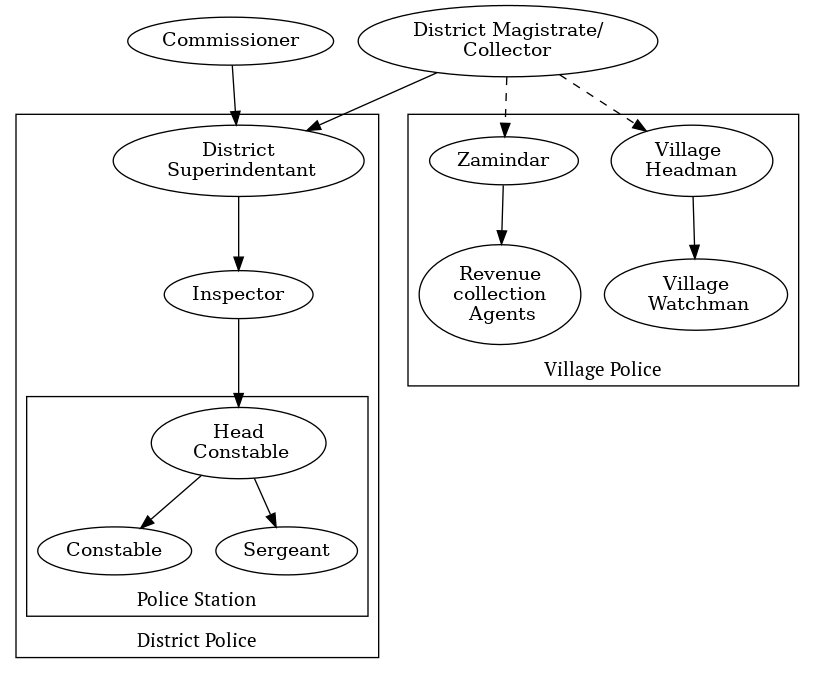
\includegraphics[width=0.8\textwidth]{police_structure}
     \end{center}
 \end{centering}

The above hierarchy is very similar to the present day system,
with the village police slowly phasing out as an unofficial
body. The deputies have been excepted in the above figure, but
provisions considering the population under the police is set in
place and implemented today across police forces in states.

The cooperation between the native population and the police
force can be concluded as a necessity for the maintenance of law
The idea that a trade company like the East India Company saw
the setup of a police organization as a priority with compelling
reasons itself indicates its importance.  and order. It is also
interesting to note how the British kept the pre-existing system
to some extent. The patient and persistent effort to improve and
develop the village police system is commendable. Also, it can
be understood that the head of the district - who today enjoys
the title of ``District Magistrate'', ``Deputy Commissioner'',
``District Collector'' all of which comes from British times for
a good reason.  It's also possible that  police and revenue
structure played an important role into converting villages into
the units of governance, as seen today. 


\printbibliography 
\end{document}
